\documentclass[a4paper,12pt]{article}
\usepackage[utf8]{inputenc}
\usepackage[ngerman]{babel}
\usepackage{amsmath}
\usepackage{mathtools}
\usepackage{float}
\usepackage{listings}
\usepackage{color}
\usepackage{graphicx}
\graphicspath{ {./pics/} }

\definecolor{pblue}{rgb}{0.13,0.13,1}
\definecolor{pgreen}{rgb}{0,0.5,0}
\definecolor{pred}{rgb}{0.9,0,0}
\definecolor{pgrey}{rgb}{0.46,0.45,0.48}

\lstdefinestyle{dsl}{
	 morekeywords={with, proxy, structproxy, for, simpleproxy, contentproxy, containerproxy, nominalproxy, provided, required, interface, extends, inject, in, posModi},
  showspaces=false,
  showtabs=false,
  breaklines=true,
   literate=
               {-->}{$\rightarrow{}$}{1}
               ,
  showstringspaces=false,
  breakatwhitespace=true,
  commentstyle=\color{pgreen},
  keywordstyle=\color{pblue},
  stringstyle=\color{pred},
   tabsize=2,
  basicstyle=\fontsize{9}{10}\selectfont\ttfamily,
  moredelim=[il][\textcolor{pgrey}]{$ $},
  moredelim=[is][\textcolor{pgrey}]{\%\%}{\%\%}
}




\newcommand{\matchTyp}[3]
{
#1  
\Rightarrow_{#2}
 #3
}

\newcommand{\methodForm}[3]
{
\mathit{#1}\texttt{ }\mathit{#2(#3)}  
}
\begin{document}

\section{Struktur für die Definition von Typen}\label{sec:strukturTypen}
Die Typen seien in einer Bibliothek $\text{L}$ in folgender Form zusammengefasst:
\begin{table}[H]
\centering
\begin{tabular}{|p{5.5cm}|p{8.5cm}|}
\hline
\hline
\centering\textbf{Regel} & \textbf{Erläuterung} \\
\hline
\hline
$\mathit{L} ::= \mathit{TD}\text{*}$ & Eine Bibliothek \emph{L} besteht aus einer Menge von Typdefinitionen.\\
\hline
$\mathit{TD} ::= \mathit{PD} | \mathit{RD}$ & Eine Typdefinition kann entweder die Definition eines provided Typen (PD) oder eines required Typen (RD) sein.\\
\hline
$\mathit{PD} ::= \newline\texttt{provided }T \texttt{ extends } T' \newline  \texttt{\{} \mathit{FD}\text{*} \mathit{MD}\text{*}\texttt{\}}$& Die Definition eines provided Typen besteht aus dem Namen des Typen \emph{T}, dem Namen des Super-Typs \emph{T'} von \emph{T} sowie mehreren Feld- und Methodendeklarationen.\\
\hline
$\mathit{RD} ::= \texttt{required } T \texttt{ \{}\mathit{MD}\text{*}\texttt{\}}$ & Die Definition eines required Typen besteht aus dem Namen des Typen \emph{T} sowie mehreren Methodendeklarationen.\\
\hline
$\mathit{FD} ::= T \texttt{ }\mathit{f}$ & Eine Felddeklaration besteht aus dem Namen des Feldes \emph{f} und dem Namen seines Typs \emph{T}.\\
\hline
$\mathit{MD} ::= \mathit{T'}\texttt{ }\mathit{m(T)}$ & Eine Methodendeklaration besteht aus dem Namen der Methode \emph{m}, dem Namen des Parameter-Typs \emph{T} und dem Namen des Rückgabe-Typs \emph{T'}.\\
\hline
\hline
\end{tabular}
\caption{Struktur für die Definition einer Bibliothek von Typen}
 \label{tab:eIShort}
\end{table}
\noindent
Weiterhin sei die Relation $<$ auf Typen durch folgende Regeln definiert:
\begin{gather*}
\frac{\texttt{provided }T \texttt{ extends } T' \in L}{T < T'}
\end{gather*}
\begin{gather*}
\frac{\texttt{provided } T \texttt{ extends } T'' \in L \wedge T'' < T'}{T < T'}
\end{gather*}

Darüber hinaus seien folgende Funktionen definiert:
\begin{gather*}
\mathit{felder(T)} :=  \left\{ 
				\begin{array}{l|l}
					T \texttt{ }\mathit{f} & T \texttt{ }\mathit{f}\text{ ist Felddeklaration von }T
				\end{array}
              \right\}\\
\mathit{methoden(T)} := \left\{ 
				\begin{array}{l|l}
					T'' \text{ }m(T') & T'' \text{ }m(T') \text{ ist Methodendeklaration von }T
				\end{array}
              \right\}\\
\mathit{feldTyp(f,T)} := 
				\begin{array}{l|l}
					T' & T' \texttt{ }\mathit{f}\text{ ist Felddeklatation von }T
				\end{array}              
\end{gather*}

\section{Beispiel-Bibliothek}



\begin{lstlisting}[style = dsl]
provided Fire extends Object{}
\end{lstlisting}

\begin{lstlisting}[style = dsl]
provided ExtFire extends Fire{}
\end{lstlisting}


\begin{lstlisting}[style = dsl]
provided FireState extends Object{
	boolean isActive
}
\end{lstlisting}

\begin{lstlisting}[style = dsl]
provided Medicine extends Object{
	String getDescription()
}
\end{lstlisting}

\begin{lstlisting}[style = dsl]
provided Injured extends Object{
	void heal(Medicine med)	
}
\end{lstlisting}


\begin{lstlisting}[style = dsl]
provided Patient extends Injured{
	String getName()
}
\end{lstlisting}
\begin{lstlisting}[style = dsl]
provided FireFighter extends Object{
	FireState extinguishFire(Fire fire)
}
\end{lstlisting}

\begin{lstlisting}[style = dsl]
provided Doctor extends Object{	
	void heal( Patient pat, Medicine med )
}
\end{lstlisting}


\begin{lstlisting}[style = dsl]
provided InverseDoctor extends Object{	
	void heal( Medicine med, Patient pat )
}
\end{lstlisting}

\begin{lstlisting}[style = dsl]
provided MedCabinet extends Object{
	Medicine med
}
\end{lstlisting}

\begin{lstlisting}[style = dsl]
required PatientMedicalFireFighter {
	void heal( Patient patient, MedCabinet med )
	boolean extinguishFire( ExtFire fire )	
}
\end{lstlisting}

\begin{lstlisting}[caption={Bibliothek \emph{ExampLe} von Typen},captionpos=b, style = dsl]
required MedicalFireFighter {
	void heal( Injured injured, MedCabinet med )
	boolean extinguishFire( ExtFire fire )	
}
\end{lstlisting}\label{lst:libEx}

\newpage

\section{Struktur für die Definition von Proxies}\label{sec:proxygram}
Die Konvertierung eines Typs $T$ aus einer Menge von provided Typen $P$ wird durch \emph{Proxies} beschrieben. Die Grammatikregeln für einen Proxies sind Tabelle \ref{tab:grProxies} zu entnehmen.
\begin{table}[H]
\centering
\begin{tabular}{|p{5cm}|p{9cm}|}
\hline
\hline
\centering\textbf{Regel} & \textbf{Erläuterung} \\
\hline
\hline
$\mathit{PROXY} ::=$\newline
$\texttt{proxy } \texttt{for } T$\newline
$ \texttt{with [}\mathit{P_1},...,\mathit{P_n}\texttt{]}$ \newline
$\texttt{\{}\mathit{MDEL_1},...,\mathit{MDEL_k} \texttt{\}}$
 & Ein Proxy wird für ein Typ $T$ als Source-Typ mit einer Mengen von provided Typen $P = \{P_1,...,P_n\}$ als Target-Typen, einer Menge von Methoden-Delegationen erzeugt.\\
\hline
$\mathit{MDEL} ::=$\newline
$CALLM \rightarrow DELM $  & Eine \emph{Methodendelegation} besteht aus einer \emph{aufgerufenen Methode} und aus einem \emph{Delegationsziel}.\\
\hline
$\mathit{CALLM} ::=$\newline 
$\mathit{REF}.\mathit{m(\mathit{CP_1},...,\mathit{CP_n}):CR} $  & Eine aufgerufene Methode besteht aus dem Namen der Methode $m$, dem Rückgabetyp $\mathit{CR}$ und einer Menge von Parametertypen $\{\mathit{CP_1},...,\mathit{CP_n}\}$.\\
\hline
$\mathit{DELM} ::=$\newline 
$\mathit{REF}.\mathit{n(\mathit{DP_1},...,\mathit{DP_n}):DR} $  
& Die erste Variante eines Delegationsziels besteht aus  dem Namen der \emph{Delegationsmethode} $n$, dem Rückgabetyp $\mathit{DR}$ und einer Menge von Parametertypen $\{\mathit{DP_1},...,\mathit{DP_n}\}$.\\
\hline
$\mathit{DELM} ::=$\newline
$\texttt{posModi(} \mathit{I_1},...,\mathit{I_n} \texttt{)}$\newline
$\mathit{REF}.\mathit{n(\mathit{DP_1},...,\mathit{DP_n}):DR} $  
& Die zweite Variante eines Delegationsziels besteht aus einer Menge von Indizies $\{\mathit{I_1},...,\mathit{I_n}\}$, einer \emph{Referenz}, dem Namen der Delegationsmethode $n$, dem Rückgabetyp $\mathit{DR}$ und einer Menge von Parametertypen $\{\mathit{DP_1},...,\mathit{DP_n}\}$.\\
\hline
$\mathit{DELM} ::= \texttt{err} $  
& Die dritte Variante eines Delegationsziels enthält keine weiteren Bestandteile. Das Terminal $\texttt{err}$ weist darauf hin, dass die Delegation innerhalb des Proxies nicht möglich ist und zu einem Fehler führt.\\
\hline
$\mathit{REF} ::= \mathit{P_i}$
& Die erste Variante einer Referenz besteht aus einem Typ $P_i$ .\\
\hline
$\mathit{REF} ::= \mathit{P_i}\texttt{.}\mathit{f}$
& Die zweite Variante einer Referenz besteht aus einem Typ $P_i$ und einem Feldnamen $f$.\\
\hline
\end{tabular}
\caption{Grammatikregeln mit Erläuterungen für die Definition eines Proxies}
 \label{tab:grProxies}
\end{table}
\noindent
Es handelt sich dabei um Produktionsregeln einer Attributgrammatik. Die dazugehörigen Attribute sind der Tabelle \ref{tab:attrGrProxies} zu entnehmen. Dazu sei zusätzlich festgelegt, dass die Notation $\mathit{NT}\texttt{.}\text{*}$ in der Spalte \emph{Attribute} eine Key-Value-Liste aller Attribute des Nonterminals $\mathit{NT}$ beschreibt, wobei der Attributname als Key und dessen Wert als Value innerhalb der Liste verwendet wird. Weiterhin sei ein Attribut, dass in der Spalte \emph{Attribute} zu einem Nonterminal nicht aufgeführt ist, wird mit dem Wert \emph{none} belegt.
\begin{table}[h!]
\centering
\begin{tabular}{|p{6cm}|p{8cm}|}
\hline
\hline
\centering\textbf{Regel} & \textbf{Attribute} \\
\hline
\hline
$\mathit{PROXY} ::=$\newline
$\texttt{proxy } \texttt{for } T$\newline
$ \texttt{with [}\mathit{P_1},...,\mathit{P_n}\texttt{]}$ \newline
$\texttt{\{}\mathit{MDEL_1},...,\mathit{MDEL_k} \texttt{\}}$
& 
$\texttt{type} = \mathit{T}$\newline
$\texttt{targets} = [\mathit{P_1},...,\mathit{P_n}]$\newline
$\texttt{dels} = [\mathit{MDEL_1}\texttt{.}\text{*},...,\mathit{MDEL_k}\texttt{.}\text{*}]$
\\
\hline
$\mathit{MDEL} ::=$\newline
$\mathit{CALLM} \rightarrow \mathit{DELM} $  
& 
$\texttt{call} = \mathit{CALLM}.*$\newline
$\texttt{del} = \mathit{DELM}.*$
\\
\hline
$\mathit{CALLM} ::=$\newline 
$\mathit{REF}.\mathit{m(\mathit{CP_1},...,\mathit{CP_n}):CR}$
& 
$\texttt{source} = \mathit{REF.\texttt{mainType}}$\newline
$\texttt{delType} = \mathit{REF.\texttt{delType}}$\newline
$\texttt{name} = \mathit{m}$\newline
$\texttt{paramTypes} = \mathit{[CP_1},...,\mathit{CP_n]}$\newline
$\texttt{returnType} = \mathit{CR}$\newline
$\texttt{field} = \mathit{REF}\texttt{.field}$\newline
$\texttt{paramCount} = n$
\\
\hline
$\mathit{DELM} ::=$\newline 
$\mathit{REF}\texttt{.}n(\mathit{DP_1},...,\mathit{DP_n}):DR $  
&
$\texttt{target} = \mathit{REF}.\texttt{mainType}$\newline
$\texttt{delType} = \mathit{REF}.\texttt{delType}$\newline
$\texttt{posModi} = [0,...,\mathit{n}-1]$\newline
$\texttt{name} = \mathit{n}$\newline
$\texttt{paramTypes} = \mathit{[DP_1},...,\mathit{DP_n]}$\newline
$\texttt{returnType} = \mathit{DR}$\newline
$\texttt{field} = \mathit{REF}\texttt{.field}$
\\
\hline
$\mathit{DELM} ::=\texttt{posModi(} \mathit{I_1},...,\mathit{I_n} \texttt{)}$\newline
$\mathit{REF}\texttt{.}n(\mathit{DP_1},...,\mathit{DP_n}):DR $  
&
$\texttt{target} = \mathit{REF}.\texttt{mainType}$\newline
$\texttt{delType} = \mathit{REF}.\texttt{delType}$\newline
$\texttt{posModi} = \mathit{[I_1},...,\mathit{I_n]}$\newline
$\texttt{name} = \mathit{n}$\newline
$\texttt{paramTypes} = \mathit{[DP_1},...,\mathit{DP_n]}$\newline
$\texttt{returnType} = \mathit{DR}$\newline
$\texttt{field} = \mathit{REF}\texttt{.field}$
\\
\hline
$\mathit{DELM} ::= \texttt{err} $  
&
\\
\hline
$\mathit{REF} ::= \mathit{P}$
& 
$\texttt{mainType} = \mathit{P}$\newline
$\texttt{field} = \texttt{self}$\newline
$\texttt{delType} = \mathit{P}$
\\
\hline
$\mathit{REF} ::= \mathit{P}\texttt{.}\mathit{f}$
&
$\texttt{mainType} = \mathit{P}$\newline
$\texttt{field} = \mathit{f}$\newline
$\texttt{delType} = \mathit{feldTyp(f,P)}$
\\
\hline
\end{tabular}
\caption{Grammatikregeln mit Attributen für die Definition eines Proxies}
 \label{tab:attrGrProxies}
\end{table}
\noindent
Ein Proxy bietet alle Methoden des Source-Typen an. Einige dieser Methoden werden an eine Methode delegiert, die von einem der Target-Typ des Proxies angeboten wird. Eine solche Delegation wird durch eine Methoden-Delegation (siehe Nontermial $\mathit{MDEL}$) definiert.
\paragraph{Beispiel} So beschreibt die folgende Methoden-Delegation, dass die Methode $\texttt{extinguishFire}$, die vom Source-Typ $\texttt{Patient}$ - und damit auch vom Proxy - angeboten wird, an die Methoden $\texttt{heal}$, die der Target-Typ $\texttt{Injured}$ anbietet, delegiert wird.
\begin{lstlisting}[style = dsl, caption = Einfache Methoden-Delegation, captionpos = b]
	Patient.heal(Medicine):void --> Injured.heal(Medicine):void
\end{lstlisting}
\noindent
Die Delegation einer aufgerufenen Methode an ein Delegationsziel, erfolgt in drei Schritten.
\begin{enumerate}
\item Parameterübergabe\\
Dabei werden die Parameter, mit denen die vom Proxy angebotene Methode, aufgerufen wird, an die Delegationsmethode des Delegationsziels übergeben. Dabei sind zwei Dinge zu beachten. Zum Einen müssen die Typen der übergebenen Parameter zu den Typen der von der Delegationsmethode erwarteten Parameter passen. Zum Anderen muss die Reihenfolge, in der die Parameter übergeben wurden, an die erwartete Reihenfolge der Delegationsmethode angepasst werden.
\item Ausführung\\
Dieser Schritt meint die Durchführung der Delegationsmethode mit den übergeben Parametern aus Schritt 1. Dies schließt auch die Ermittlung des Rückgabewertes der Delegationsmethode ein.
\item Übergabe des Rückgabewertes\\
Ähnlich wie bei der Parameterübergabe, muss auch der Rückgabewert, der bei der Ausführung in Schritt 2 ermittelt wurde, an die aufgerufenen Methode, die vom Proxy angeboten wird, übergeben werden. Hier muss ebenfalls sichergestellt werden, dass die beiden Rückgabetypen der beiden Methoden zueinander passen.
\end{enumerate}
Die Delegation aus dem oben genannten Beispiel kann schematisch wie in Abbildung \ref{fig:DEL_heal} dargestellt werden. Die Übergabe der Parameter- und Rückgabewerte wird durch die gestrichelten Pfeile symbolisiert.
\begin{figure}[h!]
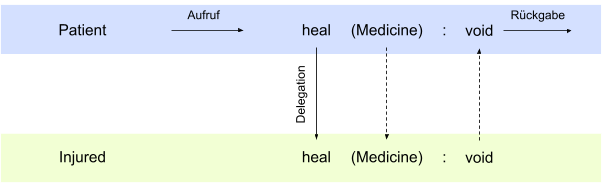
\includegraphics[width=\linewidth]{MDEL_heal}
\caption{Delegation der Methode $\texttt{heal}$}
\label{fig:DEL_heal}
\end{figure}
\noindent
An diesem Beispiel sind sowohl die Parameter- als auch die Rückgabe-Typen der aufgerufenen Methode und der Delegationsmethode identisch sind. Weiterhin spielt die Reihenfolge der Parameter in diesem Beispiel keine Rolle, da es nur einen Parameter gibt. Daher stellt die Übergabe der Parameter- und Rückgabewerte kein Problem dar.\\\\
Folgendes Beispiel soll zeigen, wie mit unterschiedlichen Reihenfolgen bzgl. der Parameter bei einer Methoden-Delegation umzugehen ist.
\paragraph{Beispiel} Die Methoden-Delegation aus Listing \ref{lst:methdel2} ist ein Beispiel für einen solchen Fall. Hier wird die aufgerufene Methode $\texttt{heal}$ mit den Parametern $\texttt{Patient}$ und $\texttt{MedCabinet}$ aus dem Typ $\texttt{PatientMedicalFireFighter}$ an die gleichnamige Methode aus dem Typ $\texttt{InverseDoctor}$ delegiert. Die Delegationsmethoden verwendet zwar identische Parameter-Typen, aber die Reihenfolge, in der die Parameter übergeben werden, ist unterschiedlich.
\begin{lstlisting}[style = dsl, caption = Methoden-Delegation mit Parametern in unterschiedlicher Reihenfolge, captionpos = b]
	PatientMedicalFireFighter.heal(Patient, MedCabinet):void --> posModi(1,0)  InverseDoctor.heal(MedCabinet,Patient):void
\end{lstlisting}\label{lst:methdel2}
\noindent
Um die Reihenfolge der Parameter aus dem ursprünglichen Aufruf zu variieren, wird das Schlüsselwort $\texttt{posModi}$ verwendet. Dort werden eine Reihe von Indizes angegeben. Die Anzahl der angegebenen Indizes muss mit der Anzahl der Parameter übereinstimmen. Ein Index beschreibt die Position des in der aufgerufenen Methode angegebenen Parameter. Weiterhin spielt die Reihenfolge der Indizes eine wichtige Rolle. Diese ist mit der Reihenfolge der Parameter der Delegationsmethoden gleichzusetzen.\\\\
So wird in dem o.g. Beispiel der erste Parameter der aufgerufenen Methoden (Index = 0) der Delegationsmethode als zweiter Parameter übergeben. Dementsprechende wird er zweite Parameter der aufgerufenen Methoden (Index = 1) der Delegationsmethode als erster Parameter übergeben (siehe Abbildung \ref{fig:DEL_healInverse}). 
\begin{figure}[H]
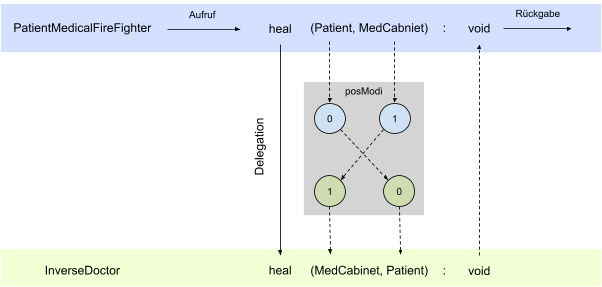
\includegraphics[width=\linewidth]{MDEL_healInverse}
\caption{Delegation der Methode $\texttt{heal}$ mit Parametern in unterschiedlicher Reihenfolge}
\label{fig:DEL_healInverse}
\end{figure}
\noindent
Ein weiteres Beispiel soll zeigen, wie mit übergebenen Typen umzugehen ist, die nicht ohne Probleme übergeben werden können. Dafür ist jedoch vorab zu klären, wann dies der Fall ist.\\\\
Dass identische Typen keine Probleme bei der Übergabe zwischen aufgerufener Methode und Delegationsmethode darstellen, wurde in den oben genannten Beispielen gezeigt.\\\\
Darüber hinaus können Typen aber auch dann ohne Probleme übergeben werden, wenn sie sich aufgrund des Substitutionsprinzips austauschen lassen. Daher kann ein Typ $T$ anstelle eines Typs $T'$ verwendet werden, sofern $T \leq T'$ gilt.
\paragraph{Beispiel} In folgendem Listing ist eine Methoden-Delegation aufgerührt, bei der sowohl die Parameter- als auch die Rückgabe-Typen der aufgerufenen Methode und der Delegationsmethode nicht auf Basis des Substitionsprinzips übergeben werden können.
\begin{lstlisting}[style = dsl, caption = Methoden-Delegation mit Typkonvertierung, captionpos = b]
	MedicalFireFighter.extinguishFire(ExtFire):boolean --> FireFigher.extinguishFire(Fire):FireState
\end{lstlisting}\label{lst:methdel3}
\noindent
In einem solchen Fall müssen die Parameter-Typen der aufgerufenen Methoden in die Parameter-Typen der Delegationsmethode konvertiert werden. Analog dazu muss der Rückgabetyp der Delegationsmethode in den Rückgabetyp der aufgerufenen Methoden konvertiert werden.\\\\
Angenommen, die Funktion $\mathit{proxies(S,T)}$ beschreibt eine Menge von Proxies, mit $S$ als Source-Typ und $T$ als Menge der Target-Typen. Dann müssten bezogen auf die Methoden-Delegation aus Listing 4 für die Parameter-Typen einer der Proxies aus der Menge $\mathit{proxies(\texttt{Fire}, \{\texttt{ExtFire}\})}$ an die Delegationsmethode übergeben werden. Nach der Ausführung der Delegationsmethode müsste ein Proxy aus der Menge $\mathit{proxies(\texttt{boolean},\{\texttt{FireState}\})}$ an die aufgerufenen Methode als Rückgabetyp übergeben werden. Der Sachverhalt wird in Abbildung \ref{fig:DEL_extinguishFire} schematisch dargestellt.
\begin{figure}[H]
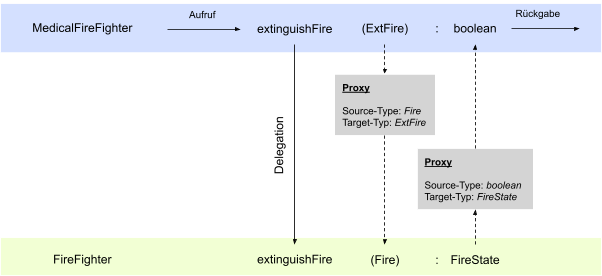
\includegraphics[width=\linewidth]{MDEL_extinguishFire}
\caption{Delegation der Methode $\texttt{extinguishFire}$ mit Typkonvertierungen}
\label{fig:DEL_extinguishFire}
\end{figure}
\noindent
Wie die Proxies generiert werden, wird im folgenden Abschnitt beschrieben.

\section{Generierung der Proxies auf Basis von Matchern}
Ein Proxy wird in Abhängigkeit vom Matching zwischen dem Source- und den Target-Typen erzeugt. Im Folgenden werden zuerst die Matcher beschrieben. Im Anschluss wird auf die Generierung der Proxies eingegangen.
\subsection{Matcher}
Ein Matcher definiert das Matching eines Typs $T$ zu einem Typ $T'$ durch die asymmetrische Relation $T \Rightarrow T'$.
\subsubsection{ExactTypeMatcher}\label{sec:exacttypematcher}
Der \emph{ExactTypeMatcher} stellt ein Matching von einem Typ $T$ zu demselben Typ $T$ her. Die dazugehörige Matchingrelation $\Rightarrow_{exact}$ wird durch folgende Regel beschrieben:
\begin{gather*}
\frac{}{T \Rightarrow_{exact} T}
\end{gather*}
\subsubsection{GenTypeMatcher}\label{sec:gentypematcher}
Der \emph{GenTypeMatcher} stellt ein Matching von einem Typ $T$ zu einem Typ $T'$ mit $T > T'$ her. Die dazugehörige Matchingrelation $\Rightarrow_{gen}$ wird durch folgende Regel beschrieben:
\begin{gather*}
\frac{T > T'}{T \Rightarrow_{gen} T'}
\end{gather*}
\subsubsection{SpecTypeMatcher}
Der \emph{SpecTypeMatcher} stellt im Verhältnis zum \emph{GenTypeMatcher} das Matching in die entgegengesetzte Richtung dar. Die dazugehörige Matchingrelation $\Rightarrow_{spec}$ wird durch folgende Regel beschrieben: 
\begin{gather*}
\frac{T < T'}{T \Rightarrow_{spec} T'}
\end{gather*}
\\\\
Die oben genannten Matchingrelationen werden für die Definition weiterer Matcher zusammengefasst, wodurch sich die Matchingrelation $\Rightarrow_{internCont}$ ergibt:
\begin{gather*}
\frac{T \Rightarrow_{exact} T' \vee T \Rightarrow_{gen} T' \vee
T \Rightarrow_{spec} T'  }{T \Rightarrow_{internCont} T'}
\end{gather*}
\subsubsection{ContentTypeMatcher}
Der \emph{ContentTypeMatcher} matcht einen Typ $T$ auf einen Typ $T'$, wobei $T'$ ein Feld enthält, auf dessen Typ $T''$ der Typ $T$ über die Matchingrelation $\Rightarrow_{internCont}$ gematcht werden kann. So kann bspw. der Typ $\texttt{boolean}$ aus Listing 1 auf den Typ $\texttt{FireState}$ gematcht werden.
\\\\
Die dazugehörige Matchingrelation $\Rightarrow_{content}$ wird durch folgende Regel beschrieben:
\begin{gather*}
\frac{\exists \mathit{T''\text{ }f}\in felder(T'): T \Rightarrow_{internCont} T''}{T \Rightarrow_{content} T'}
\end{gather*}
\noindent
So würde für die Typen $\texttt{boolean}$ und $\texttt{FireState}$ gelten: 
\begin{gather*}
\texttt{boolean} \Rightarrow_{content} \texttt{FireState}
\end{gather*}
\subsubsection{ContainerTypeMatcher}
Der \emph{ContainerTypeMatcher} stellt im Verhältnis zum \emph{ContentTypeMatcher} das Matching in die entgegengesetzte Richtung dar. So kann bspw. auch der Typ $\texttt{FireState}$ auf den Typ $\texttt{booealn}$ aus Listing 1 gematcht werden.
\\\\
Die dazugehörige Matchingrelation $\Rightarrow_{container}$ wird durch folgende Regel beschrieben:
\begin{gather*}
\frac{\exists \mathit{T''\text{ }f}\in felder(T): T'' \Rightarrow_{internCont} T'}{T \Rightarrow_{container} T'}
\end{gather*}
\noindent
So gilt für die Typen $\texttt{FireState}$ und $\texttt{boolean}$: 
\begin{gather*}
\texttt{FireState} \Rightarrow_{container} \texttt{boolean}
\end{gather*}
\\\\
Zur Definition des letzten Matchers werden die Matchingrelationen der oben genannten Matcher noch einmal zusammengefasst. Dabei entsteht die Matchingrelation $\Rightarrow_{internStruct}$, welche durch folgende Regel beschrieben wird:
\begin{gather*}
\frac{T \Rightarrow_{internCont}T' \vee T \Rightarrow_{container} T' \vee T \Rightarrow_{content} T'}{T \Rightarrow_{internStruct}T'}
\end{gather*}
\subsubsection{StructuralTypeMatcher} 
Der \emph{StructuralTypeMatcher} matcht einen \emph{required Typ} $R$ auf einen \emph{provided Typ} $P$ auf der Basis struktureller Eigenschaften der Methoden, die in den Typen deklariert sind. 
\\\\
Somit soll bspw. der Typ $\texttt{MedicalFireFighter}$ auf den Typ $\texttt{FireFighter}$ (siehe Listing 1) gematcht werden. Als ein weiteres Beispiel, bezogen auf die Typen aus Listing 1, kann das Matching des Typs $\texttt{MedicalFireFighter}$ auf den Typ $\texttt{Doctor}$ angebracht werden.
\\\\
Damit ein required Typ $R$ auf einen provided Typ $P$ über den \emph{StrukturalTypeMatcher} gematcht werden kann, muss mindestens eine Methode aus $R$ zu einer Methode aus $P$ gematcht werden. Die Menge der gematchten Methoden aus $R$ in $P$ wird wie folgt beschrieben:
\begin{gather*}
structM(R,P) := \left\{ 
				\begin{array}{l|l}
				& \mathit{T'\text{ }m(T)} \in \mathit{methoden(R)} \wedge \mathit{ }\\
T'\text{ }m(T)	& \exists \mathit{S'\text{ }n(S)} \in \mathit{methoden(P)} :\\								 				&  S\Rightarrow_{internStruct}T \wedge T' \Rightarrow_{internStruct}S' 
				\end{array}
              \right\}
\end{gather*}
Da die Notation es nicht hergibt, ist zusätzlich zu erwähnen, dass, sofern in $m$ und $n$ mehrere Parameter verwendet werden, deren Reihenfolge irrelevant ist.\\\\
Die Matchingrelation für die \emph{StructuralTypeMatcher} wird durch folgende Regel beschrieben:
\begin{gather*}
\frac{structM(R,P) \neq \emptyset}{R \Rightarrow_{struct}P}
\end{gather*}
\subsection{Generierung von Proxies}
Wie im Abschnitt \ref{sec:proxygram} bereits erwähnt, soll die Menge der Proxies für einen Source-Typ $S$ und einer Menge von Target-Typen $T$ über die Funktion $\mathit{proxies(S,T)}$ beschrieben werden.\\\\
In Abhängigkeit von dem Matching zwischen dem Source-Typ und den Target-Typen werden unterschiedliche Arten von Proxies generiert. Für die unterschiedlichen Proxy-Arten gibt es ebenfalls Funktionen, die eine Menge von Proxies zu einem Source-Typen $S$ und einer Menge von Target-Typen $T$ beschreiben.\\\\
In den folgenden Abschnitten werden diese Funktionen für die einzelnen Proxy-Arten beschrieben. Dabei ist davon auszugehen, dass die Proxies eine allgemeine Struktur haben, die in Abschnitt \ref{sec:proxygram} aufgeführt ist. Um die Regeln für die Generierung der Proxies zu beschreiben, soll davon ausgegangen werden, dass jedes Listen-Attribut ($\mathit{NT.}\text{*}$) aus Tabelle \ref{tab:attrGrProxies} ein Attribut $\texttt{len}$ enthält in dem die Anzahl der in der Liste befindlichen Elemente abgelegt ist.


\subsubsection{Sub-Proxy}
Die Voraussetzung für die Erzeugung eines \emph{Sub-Proxies} vom Typ $T$ aus einem Target-Typ $T'$ ist $T \Rightarrow_{spec} T'$. Damit ist der \emph{SpecTypeMatcher} der Basis-Matcher für den Sub-Proxy.
\paragraph{Beispiel}
Als Beispiel soll  der Typ $\texttt{Patient}$ als Source-Typ und der Typ $\texttt{Injured}$ als Target-Typ verwendet werden. Da $\texttt{Patient} \Rightarrow_{spec} \texttt{Injured}$ gilt, kann ein \emph{Sub-Proxy} für diese Konstellation erzeugt werden. Der resultierende \emph{Sub-Proxy} ist im folgenden Listing aufgeführt.
\begin{lstlisting}[style = dsl, caption = Sub-Proxy für Patient, captionpos = b]
proxy for Patient with [Injured]{
	Patient.heal(Medicine):void --> Injured.heal(Medicine):void
	Patient.getName():String --> err
}
\end{lstlisting}
Der abstrakte Syntaxbaum mit den dazugehörigen Attributen ist Abbildung \ref{fig:ASTSUB} zu entnehmen. \footnote{Es wurden nur die Nonterminale mit den dazugehörigen Attributen aufgeführt.}
\begin{figure}[h!]
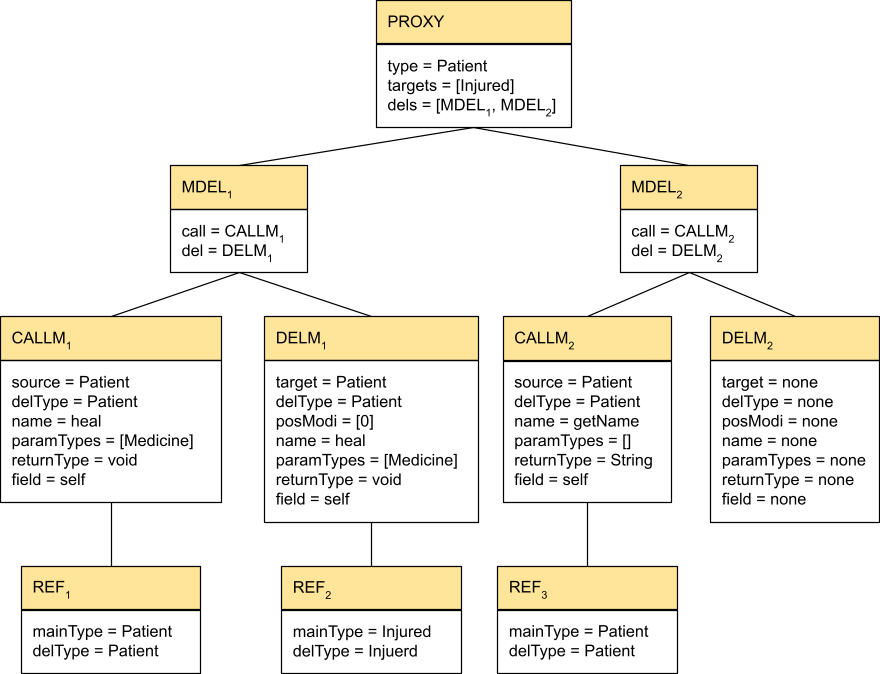
\includegraphics[width=\linewidth]{AST_SubExample}
\caption{AST für das Beispiel zum Sub-Proxy}
\label{fig:ASTSUB}
\end{figure}
\noindent
Der Proxy bietet alle Methoden an, die auch von dessen Source-Typ angeboten werden. Die Methodendelegationen innerhalb des Proxies, beschreiben, was beim Aufruf der jeweiligen aufgerufenen Methoden passiert. So wird ein Aufruf der Methode $\texttt{heal}$ an die Methode $\texttt{heal}$ aus dem Target-Typ delegiert. Ein Aufruf der Methode $\texttt{getName}$ hingegen führt zu einem Fehler, weil keine Delegationsmethode zur Verfügung steht.\\\\
Im Hinblick darauf, dass eine Konvertierung von einem Super-Typ und einen Sub-Typ (Down-Cast) ebenfalls dazu führt, dass bestimmte Methoden, wie in diesem Fall $\texttt{getName}$ nicht ausgeführt werden können, spiegelt der \emph{Sub-Proxy} dieses Verhalten wieder.
\paragraph{Formalisierung}
Formal wird ein \emph{Sub-Proxy} durch die Regeln beschrieben, die im Folgenden vorgestellt werden. Ein \emph{Sub-Proxy} enthält genau einen Target-Typ. Für einen Proxy $P$ wird dieser Sachverhalt durch die folgende Regel dargestellt.
\begin{gather*}
\frac{|\mathit{P.targets}| = 1 \wedge \forall \mathit{T'} \in \mathit{P.targets}: T = T'}{\mathit{targets_{single}(P,T)}}
\end{gather*}
Darüber hinaus enthält ein \emph{Sub-Proxy} $P$ eine bestimmte Menge von Methoden-Delegationen. Dabei muss in allen Methodendelegationen das Attribut $\texttt{field}$ der aufgerufenen Methoden mit dem der Delegationsmethoden übereinstimmen. Folgende Regel stellt diesen Sachverhalt für eine Menge von Methoden-Delegationen $\mathit{MDList}$ dar.
\begin{gather*}
\frac{\splitfrac{\forall \mathit{MD_1}\in \mathit{MDList}: \neg(\exists \mathit{MD_2} \in \mathit{MDList}:\mathit{MD_1.call.field} \neq \mathit{MD_2.call.field}}{ \vee \mathit{MD_1.del.field} \neq \mathit{MD_2.del.field} )}}
{\mathit{equalRefs(MDList)}}
\end{gather*}
Für jede einzelne Methoden-Delegation $\mathit{MD}$ gilt weiterhin, dass die aufgerufene Methode und die Delegationsmethode denselben Namen haben.
\begin{gather*}
\frac{\mathit{MD.call.name} = \mathit{MD.del.name}}
{\mathit{methDel_{nominal}(MD)}}
\end{gather*}
Die aufgerufene Methode muss dabei generell im Typ aus dem Attribut $\texttt{call.delType}$ deklariert sein und die Delegationsmethode im Typ aus dem Attribut $\texttt{del.delType}$.
\begin{gather*}
\frac{\exists \mathit{T'\text{ } m(T)} \in \mathit{methoden(MD.call.delType)}: \mathit{MD.call.name} = m}
{\mathit{callMethod_{simple}(MD)}}
\end{gather*}
\begin{gather*}
\frac{\exists \mathit{T'\text{ }m(T)} \in \mathit{methoden(MD.del.delType)}: \mathit{MD.del.name} = m}
{\mathit{delMethod_{simple}(MD)}}
\end{gather*}
Zusätzlich muss das Attribut $\texttt{field}$ im Attribut $\texttt{call}$ mit dem Wert $\texttt{self}$ belegt und das Attribut $\texttt{mainType}$ mit dem Source-Typ des Proxies belegt sein.
\begin{gather*}
\frac{\mathit{MD.call.mainType} = \mathit{P.type} \wedge \mathit{MD.call.field} = \mathit{self}}
{\mathit{callMethodDelType_{simple}(MD, P)}}
\end{gather*}
Damit ist auch automatisch gewährleistet, dass die Attribute $\texttt{mainType}$ und $\texttt{delType}$ im Attribut $\texttt{call}$ übereinstimmen. (siehe Tabelle \ref{tab:attrGrProxies})\\\\
Ähnliches gilt für die Attribute $\texttt{field}$ und $\texttt{mainType}$ im Attribut $\texttt{del}$. Hierbei muss der Wert des Attributs $\texttt{mainType}$ jedoch mit dem Target-Typ des Proxies übereinstimmen.
\begin{gather*}
\frac{\mathit{MD.del.field} = \mathit{self} \wedge  \mathit{MD.del.mainType} \in \mathit{P.targets} }
{\mathit{delMethodDelType_{simple}(MD, P)}}
\end{gather*}
Damit ist wiederum automatisch gewährleistet, dass die Attribute $\texttt{mainType}$ und $\texttt{delType}$ im Attribut $\texttt{del}$ übereinstimmen. (siehe Tabelle \ref{tab:attrGrProxies})\\\\
Die Regeln für die linke Seite einer Methoden-Delegation $\mathit{MD}$ innerhalb eines \emph{Sub-Proxies} $P$ können damit in folgender Regel zusammengefasst werden:
\begin{gather*}
\frac{\mathit{callMethod_{simple}(MD)} \wedge \mathit{callMethodDelType_{simple}(MD,P)}}
{\mathit{call_{simple}(MD,P)}}
\end{gather*}
Analog dazu können auch die Regeln für die rechte Seite einer Methoden-Delegation $\mathit{MD}$ innerhalb eines \emph{Sub-Proxies} $P$ zusammengefasst werden:
\begin{gather*}
\frac{\mathit{delMethod_{simple}(MD)} \wedge \mathit{delMethodDelType_{simple}(MD,P)}}
{\mathit{del_{simple}(MD,P)}}
\end{gather*}
Im \emph{Sub-Proxy} ist darüber hinaus noch die Methoden-Delegation zu beachten, die bei einem Aufruf zu einem Fehler führt. Dieser Fall wird für eine Methoden-Delegation $\mathit{MD}$ wie folgt beschrieben:
\begin{gather*}
\frac{\mathit{MD.del.name} = \mathit{none}}
{\mathit{del_{err}(MD)}}
\end{gather*}
Die genannten Regeln für eine Methoden-Delegation $\mathit{MD}$ in einem \emph{Sub-Proxy} lassen sich über die beiden folgenden Regeln beschreiben:
\begin{gather*}
\frac{\mathit{call_{simple}(MD,P)} \wedge \mathit{del_{simple}(MD,P) \wedge \mathit{methDel_{nominal}(MD)}}}
{\mathit{methDel_{sub}(MD,P)}}
\end{gather*}
\begin{gather*}
\frac{\mathit{call_{simple}(MD,P)}\wedge\mathit{del_{err}(MD)}
}
{\mathit{methDel_{sub}(MD,P)}}
\end{gather*}
Innerhalb eines \emph{Sub-Proxies} gibt es für jede Methode $m$ des Source-Typ genau eine Methoden-Delegation mit der Methode $m$ als aufgerufene Methode. Damit lässt sich für einen Proxy $P$ in Bezug auf alle seine Methoden-Delegationen folgende Regeln formulieren:
\begin{gather*}
\frac{\splitfrac{\mathit{M} = \mathit{methoden(P.type)}\wedge|\mathit{M}| = |P.dels| \wedge \forall \mathit{T'\text{ }m(T)} \in \mathit{M}:}{\exists \mathit{MD} \in \mathit{P.dels}:m = \mathit{MD.call.name} \wedge \mathit{methDel_{sub}(MD,P)
 }}
}
{\mathit{methDelList_{sub}(P)}}
\end{gather*}
Für einen Proxy $P$ kann die Regel $\mathit{equalRefs(P)}$ im Allgemeinen mit der Bedingung zusammengefasst werden, die besagt, dass ein Proxy immer einen bestimmten Source-Typ $S$ haben muss. Die zusammengefasste Regel lautet:
\begin{gather*}
\frac{\mathit{P.type} = \mathit{S} \wedge \mathit{equalRefs(P)}}{\mathit{proxy(P,S)}}
\end{gather*}
\noindent
Die Menge der \emph{Sub-Proxies}, die mit dem Source-Typ $T$ und dem Target-Typ $T'$ erzeugt werden, wird durch die folgende Funktion beschrieben.
\begin{gather*}
\mathit{proxies_{sub}(T,T')} := 
\left\{\begin{array}{l|l}
		& \mathit{proxy(P,T)}\wedge \mathit{ } \\
	P	& \mathit{targets_{single}(P,T')} \wedge \mathit{ } \\
		& \mathit{methDelList_{sub}(P)}
		 \end{array}
\right\}
\end{gather*}


\subsubsection{Content-Proxy}
Die Voraussetzung für die Erzeugung eines \emph{Content-Proxies} vom Typ $T$ aus einem Target-Typ $T'$ ist $T \Rightarrow_{content} T'$. Damit ist der \emph{ContentTypeMatcher} der Basis-Matcher für den \emph{Content-Proxy}.
\paragraph{Beispiel} Als Beispiel sollen die Typen $\texttt{Medicine}$ und $\texttt{MedCabinet}$ verwendet werden, welche ein Matching der Form $\texttt{Medicine} \Rightarrow_{content} \texttt{MedCabinet}$ aufweisen. Daher kann ein \emph{Content-Proxy} für diese Konstellation erzeugt werden. Ein resultierender \emph{Content-Proxy} ist in folgendem Listing aufgeführt.
\begin{lstlisting}[style = dsl, caption = Content-Proxy für Medicine, captionpos = b]
proxy for Medicine with [MedCabinet]{
	Medicine.getDesciption():String --> MedCabinet.med.getDesciption():String
}
\end{lstlisting}
Durch die Methoden-Delegation dieses \emph{Content-Proxies} wird die Methode $\texttt{getDescription}$ an das Feld $\texttt{med}$ des Target-Typen $\texttt{MedCabniet}$ delegiert.\\\\
Der abstrakte Syntaxbaum mit den dazugehörigen Attributen ist Abbildung \ref{fig:ASTCONTENT} zu entnehmen. \footnote{Es wurden nur die Nonterminale mit den dazugehörigen Attributen aufgeführt.}
\begin{figure}[h!]
\centering
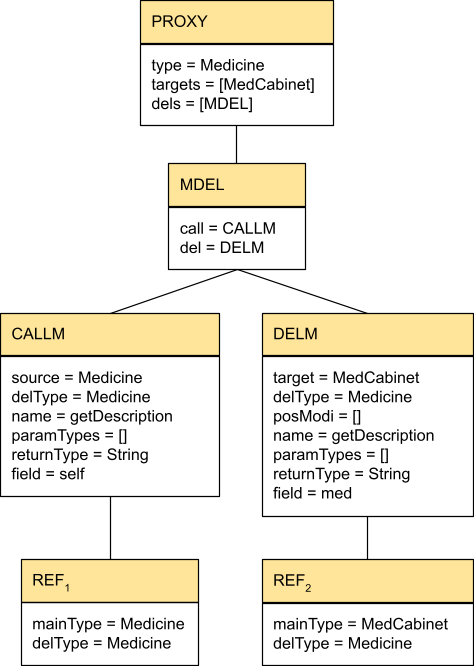
\includegraphics[width=0.5\linewidth]{AST_ContentExample}
\caption{AST für das Beispiel zum Content-Proxy}
\label{fig:ASTCONTENT}
\end{figure}
\noindent
\paragraph{Formalisierung}
Formal wird ein \emph{Content-Proxy} durch die Regeln beschrieben, die im Folgenden vorgestellt werden.\\\\
Ein \emph{Content-Proxy} enthält, wie auch der \emph{Sub-Proxy}, genau einen Target-Typ. Ebenfalls identisch zum \emph{Sub-Proxy} sind die Bedingungen hinsichtlich der aufgerufenen Methoden in den einzelnen Methoden-Delegationen.\\\\
In den Delegationsmethoden einer einzelnen Methoden-Delegation $\mathit{MD}$ dürfen die Attribute $\texttt{mainType}$ und $\texttt{delType}$ im \emph{Content-Proxy} nicht identisch sein. Dementsprechend darf das Attribut $\texttt{field}$ nicht mit dem Wert $\texttt{self}$ belegt sein. Vielmehr muss für das Attribut $\texttt{delTyp}$ und den Source-Typ $T$ des Proxies ein Matching der Form $T \Rightarrow_{internCont} \mathit{MD.del.delTyp}$ gelten. Daher gilt für den \emph{Content-Proxy} die folgende Regel:
\begin{gather*}
\frac{\mathit{P.type} \Rightarrow_{internCont} \mathit{MD.del.delType}  \wedge \mathit{MD.del.mainType} \in \mathit{P.targets}}
{\mathit{delMethodDelType_{content}(MD,P)}}
\end{gather*}
\noindent
Damit kann eine zusammenfassende Regel für die Delegationsmethoden einer Methoden-Delegation $\mathit{MD}$ wie folgt definiert werden:
\begin{gather*}
\frac{\mathit{delMethod_{simple}(MD)} \wedge \mathit{delMethodDelType_{content}(MD,P)}}
{\mathit{del_{content}(MD,P)}}
\end{gather*}
Die zusammenfassende Regel für eine einzelne Methoden-Delegation $\mathit{MD}$ innerhalb eines \emph{Content-Proxies} hat die folgende Form:
\begin{gather*}
\frac{\mathit{call_{simple}(MD,P)} \wedge \mathit{del_{content}(MD,P) \wedge \mathit{methDel_{nominal}(MD)}}}
{\mathit{methDel_{content}(MD,P)}}
\end{gather*}
Wie auch im \emph{Sub-Proxy} gibt es im \emph{Content-Proxy} für jede Methode $m$ des Source-Typen genau eine Methoden-Delegation mit der Methode $m$ als aufgerufene Methode. Daraus ergibt sich für alle Methoden-Delegationen aus einem \emph{Content-Proxy} $P$ folgende Regel:
\begin{gather*}
\frac{\splitfrac{M = \mathit{methoden(P.type) }\wedge|\mathit{M}| = |\mathit{P.dels}| \wedge \forall \mathit{T' \text{ }m(T)} \in \mathit{M}:}{ \exists \mathit{MD} \in \mathit{P.dels}:m = \mathit{MD.call.name} \wedge \mathit{methDel_{content}(MD,P)
 }
}}
{methDelList_{content}(P)}
\end{gather*}
Die Menge der \emph{Content-Proxies}, die mit dem Source-Typ $T$ und dem Target-Typ $T'$ erzeugt werden, wird durch die folgende Funktion beschrieben.
\begin{gather*}
\mathit{proxies_{content}(T,T')} := 
\left\{\begin{array}{l|l}
		& \mathit{proxy(P,T)} \wedge \mathit{ } \\
	P	& \mathit{targets_{single}(P,T')} \wedge \mathit{ }\\
		& \mathit{methDelList_{content}(P)} 
		 \end{array}
\right\}
\end{gather*}
\subsubsection{Container-Proxy}
Die Voraussetzung für die Erzeugung eines \emph{Container-Proxies} vom Typ $T$ aus einem Target-Typ $T'$ ist $T \Rightarrow_{container} T'$. Damit ist der \emph{ContainerTypeMatcher} der Basis-Matcher für den \emph{Container-Proxy}.
\paragraph{Beispiel}
Als Beispiel werden wiederum die Typen $\texttt{Medicine}$ und $\texttt{MedCabinet}$ verwendet, welche ein Matching der Form $\texttt{MedCabinet} \Rightarrow_{container} \texttt{Medicine}$ aufweisen. Daher kann ein \emph{Content-Proxy} für diese Konstellation erzeugt werden. Ein resultierender \emph{Content-Proxy} ist in folgendem Listing aufgeführt.
\begin{lstlisting}[style = dsl, caption = Container-Proxy für MedCabniet, captionpos = b ]
proxy for MedCabinet with [Medicine]{
	MedCabinet.med.getDesciption():String --> Medicine.getDesciption():String
}
\end{lstlisting}
Durch die Methoden-Delegation dieses \emph{Container-Proxies} findet eine Delegation nur dann statt, wenn die Methoden $\texttt{getDescription}$ auf dem Feld $\texttt{med}$ des Source-Typ aufgerufen wird. Diese wird dann an den Target-Typen $\texttt{MedCabniet}$ delegiert.\\\\
Der abstrakte Syntaxbaum mit den dazugehörigen Attributen ist Abbildung \ref{fig:ASTCONTAINER} zu entnehmen. \footnote{Es wurden nur die Nonterminale mit den dazugehörigen Attributen aufgeführt.}
\begin{figure}[h!]
\centering
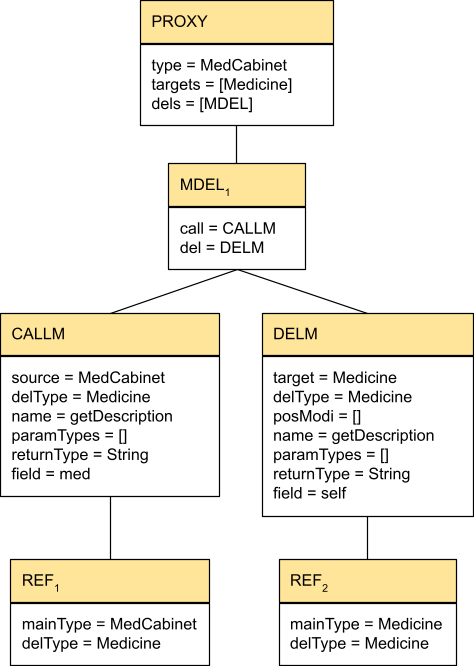
\includegraphics[width=0.5\linewidth]{AST_ContainerExample}
\caption{AST für das Beispiel zum Container-Proxy}
\label{fig:ASTCONTAINER}
\end{figure}
\noindent
\paragraph{Formalisierung}
Formal wird ein \emph{Container-Proxy} durch die Regeln beschrieben, die im Folgenden vorgestellt werden.\\\\
Ein \emph{Container-Proxy} enthält, wie die vorher beschriebenen Proxies, genau einen Target-Typ. Die Eigenschaften der Delegationsmethoden innerhalb der einzelnen Methoden-Delegationen gleichen denen aus dem \emph{Sub-Proxy}.\\\\
In den angerufenen Methoden einer einzelnen Methoden-Delegation $\mathit{MD}$ dürfen die Attribute $\texttt{mainType}$ und $\texttt{delType}$ im \emph{Container-Proxy} nicht übereinstimmen. Dementsprechend darf das Attribut $\texttt{field}$ nicht mit dem Wert $\texttt{self}$ belegt sein. Vielmehr müssen der Wert des Attributs $\texttt{delTyp}$ und der Target-Typ $T$ des Proxies ein Matching der Form $T \Rightarrow_{internCont} \texttt{delTyp}$ ausweisen. Daher gilt für den \emph{Container-Proxy} $P$ folgende Regel.
\begin{gather*}
\frac{\splitfrac{\mathit{MD.call.mainType} = \mathit{P.type} \wedge \forall \mathit{T} \in \mathit{P.targets}:}
{  \mathit{T} \Rightarrow_{internCont} \mathit{MD.call.delType}}
}
{\mathit{callMethodDelType_{container}(MD,P)}}
\end{gather*}
\noindent
Damit kann eine zusammenfassende Regel für die aufgerufenen Methoden wie folgt definiert werden:
\begin{gather*}
\frac{\mathit{callMethod_{simple}(MD)} \wedge \mathit{callMethodDelType_{container}(MD,P)}}
{\mathit{call_{container}(MD,P)}}
\end{gather*}
Die zusammenfassende Regel für eine einzelne Methoden-Delegation $\mathit{MD}$ innerhalb eines \emph{Container-Proxies} hat die folgende Form:
\begin{gather*}
\frac{\mathit{call_{container}(MD,P)} \wedge \mathit{del_{simple}(MD,P)} \wedge \mathit{methDel_{nominal}(MD)}}
{\mathit{methDel_{container}(MD,P)}}
\end{gather*}
Für einen \emph{Container-Proxy} $P$ gilt ebenfalls die Regel $\mathit{equalRefs(P.dels)}$. Daher müssen die Werte des Attributs $\texttt{call.delType}$ aller Methoden-Delegationen des Proxies $P$ übereinstimmen. Ferner muss es für jede Methode $m$ des Typen aus $\texttt{call.delType}$ genau eine Methoden-Delegation mit der Methode $m$ als aufgerufene Methode existieren. Daraus ergibt sich für alle Methoden-Delegationen aus einem \emph{Content-Proxy} $P$ folgende Regel:
\begin{gather*}
\frac{\splitfrac{\mathit{M} = \mathit{methoden(P.dels[0].call.delType)} \wedge |\mathit{M}| = |P.dels| \wedge \forall \mathit{T' \text{ } m(T)} \in \mathit{M}:}
{\exists \mathit{MD} \in P.dels:m = \mathit{MD.call.name} \wedge \mathit{methDel_{container}(MD,P)}
 }}
{\mathit{methDelList_{container}(P)}}
\end{gather*}
Die Menge der \emph{Container-Proxies}, die mit dem Source-Typ $T$ und dem Target-Typ $T'$ erzeugt werden, wird durch die folgende Funktion beschrieben.
\begin{gather*}
\mathit{proxies_{container}(T,T')} := 
\left\{\begin{array}{l|l}
		& \mathit{proxy(P,T)}  \wedge \mathit{ } \\
	P	& \mathit{target_{single}(P,T')} \wedge \mathit{ } \\
		& \mathit{methDelList_{container}(P)} 
		 \end{array}
\right\}
\end{gather*}

\subsubsection{Struktureller Proxy}
Die Voraussetzung für die Erzeugung eines \emph{strukturellen Proxies} vom \emph{required Typ} $R$ aus einem Target-Typ $T$ ist $R \Rightarrow_{struct} T$. Damit ist der \emph{StructuralTypeMatcher} der Basis-Matcher für den \emph{strukturellen Proxy}.\\\\
Der \emph{strukturelle Proxy} ist der einzige Proxy, der mit mehreren Target-Typen erzeugt werden kann. 
\paragraph{Beispiel}
Als Beispiel werden die Typen $\texttt{MedicalFireFighter}$, $\texttt{Doctor}$ und $\texttt{FireFighter}$ verwendet. Dabei ist $\texttt{MedicalFireFighter}$ der Source-Typ des Proxies und die Menge der anderen beiden Typen bilden die Target-Typen des Proxies. Da der Source-Typ zu den Target-Typen ein Matching der Form $\texttt{MedicalFireFighter} \Rightarrow_{struct} \texttt{FireFighter}$ bzw. $\texttt{MedicalFireFighter} \Rightarrow_{struct} \texttt{Doctor}$ aufweist, kann ein \emph{struktureller Proxy} erzeugt werden. Ein solcher ist in folgendem Listing aufgeführt.
\begin{lstlisting}[style = dsl, caption = Struktureller Proxy für MedicalFireFighter, captionpos = b]
proxy for MedicalFireFighter with [Doctor, FireFighter]{
	MedicalFireFighter.heal(Patient, MedCabinet):void --> Doctor.heal(Patient, Medicine):void
	MedicalFireFighter.extinguishFire(ExtFire):boolean --> FireFighter.extinguishFire(Fire):FireState
}
\end{lstlisting}
In diesem Beispiel wird der Methodenaufruf der Methode $\texttt{heal}$ auf dem Proxy an die Methode $heal$ des Typs $\texttt{Doctor}$ delegiert. Analog dazu würde ein Aufruf der Methode $\texttt{extinguishFire}$ auf dem Proxy an die Methode $extinguishFire$ des Typs $\texttt{FireFighter}$ delegiert werden. Die Methoden stimmen jeweils strukturell überein.\\\\
Der abstrakte Syntaxbaum mit den dazugehörigen Attributen ist Abbildung \ref{fig:ASTSTRUCT} zu entnehmen. \footnote{Es wurden nur die Nonterminale mit den dazugehörigen Attributen aufgeführt.}
\begin{figure}[h!]
\centering
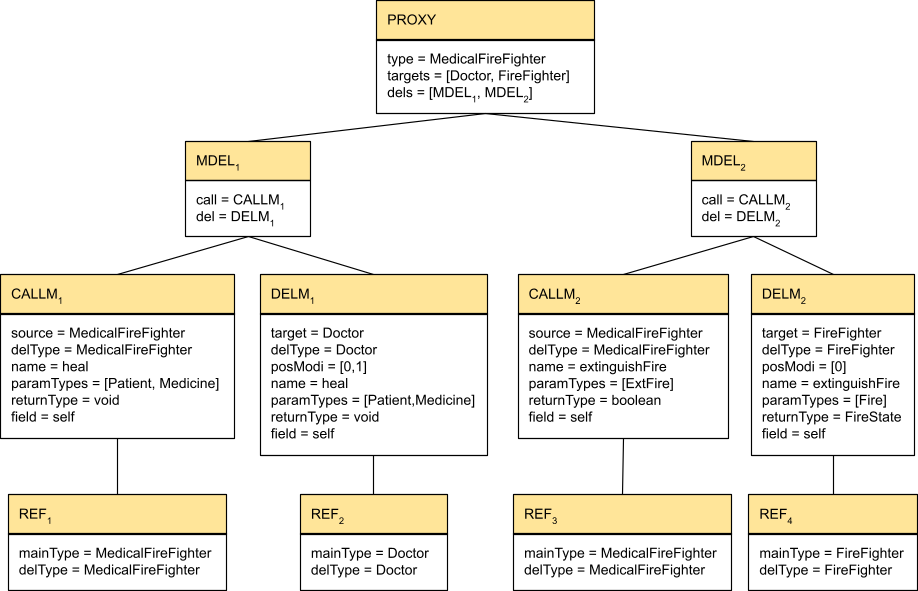
\includegraphics[width=\linewidth]{AST_StructExample}
\caption{AST für das Beispiel zum strukturellen Proxy}
\label{fig:ASTSTRUCT}
\end{figure}
\noindent
\paragraph{Formalisierung}
Ein \emph{struktureller Proxy} wird formal durch die folgenden Regeln beschrieben.\\\\
Ein \emph{struktureller Proxy} kann, wie bereits erwähnt, mehrere Target-Typen enthalten.
Für jeden Target-Typ $T$ muss dabei jedoch wenigstens eine Delegationsmethode im Proxy mit einem Attribut $\texttt{target} = T$ existiert. Dadurch gilt die für einen \emph{strukturellen Proxy} Proxy $P$:
\begin{gather*}
\frac{\forall \mathit{T} \in \mathit{P.targets}:\exists \mathit{MD} \in \mathtt{P.dels}:\mathit{MD.del.target} = T}{\mathit{targets_{struct}(P, T)}}
\end{gather*}
Für die aufgerufene Methode und die Delegationsmethode einer einzelnen Methoden-Delegation $\mathit{M}$ gelten im \emph{strukturellen Proxy} dieselben Regeln wie für den \emph{Sub-Proxy}. Die Namen der aufgerufenen Methode und der Delegationsmethode müssen dabei jedoch nicht übereinstimmen. Dafür müssen diese beiden Methode jedoch ein strukturelles Matching aufweisen. Bezogen auf die Rückgabe-Typen einer aufgerufenen Methode $\mathit{C}$ und der Delegationsmethode $\mathit{D}$ aus einer Methoden-Delegation muss daher Folgendes gelten.
\begin{gather*}
\frac{\mathit{D.returnType} \Rightarrow_{internStruct} \mathit{C.returnType}}{\mathit{return_{struct}(C,D)}}
\end{gather*} 
Weiterhin muss für die Parameter-Typen gelten:
\begin{gather*}
\frac{\mathit{C.paramCount} = 0}{\mathit{params_{struct}(C,D)}}
\end{gather*} 
\begin{gather*}
\frac{\splitfrac{\forall \mathit{i} \in \{0,...,\mathit{C.paramCount}-1\}:}
{ \mathit{C.paramTypes}[i] \Rightarrow_{internStruct} \mathit{D.paramTypes}[\mathit{D.posModi}[i]]
}}{\mathit{params_{struct}(C,D)}}
\end{gather*} 
Für eine einzelne Methoden-Delegation $\mathit{MD}$ eines \emph{strukturellen Proxies} $P$ kann dann folgende Regel aufgestellt werden.
\begin{gather*}
\frac{\splitfrac{\mathit{call_{simple}(MD,P)} \wedge \mathit{del_{simple}(MD,P)} \wedge} {\mathit{return_{struct}(MD.call, MD.del)} \wedge \mathit{params_{struct}(MD.call, MD.del)}}
}
{\mathit{methDel_{struct}(MD,P)}}
\end{gather*}
In einem \emph{strukturellen Proxy} muss für jede Methode $m$ des Source-Typen genau eine Methoden-Delegation mit der Methode $m$ als aufgerufene Methode existieren. Daraus ergibt sich für alle Methoden-Delegationen aus einem \emph{strukturellen Proxy} $P$ folgende Regel:
\begin{gather*}
\frac{\splitfrac{\mathit{M} = \mathit{methoden(P.type)} \wedge |\mathit{M}| = |\mathit{P.dels}| \wedge \forall \mathit{T' \text{ }m(T)} \in \mathit{M}:}{\exists \mathit{MD} \in \mathit{P.dels}:\mathit{MD.call.name} = m \wedge \mathit{methDel_{struct}(MD,P)}
 }
}
{\mathit{methDelList_{struct}(P)}}
\end{gather*}
Wie in Abschnitt 
Die Menge der \emph{strukturellen Proxies}, die mit dem Source-Typ $R$ und der Menge von Target-Typen $T$ erzeugt werden, wird durch die folgende Funktion beschrieben.
\begin{gather*}
\mathit{proxies_{struct}(R,T)} := 
\left\{\begin{array}{l|l}
		& \mathit{proxy(P,R)}\wedge \mathit{ }\\
	P	& \mathit{targets_{struct}(P,T)} \wedge \mathit{ }\\
		& \mathit{methDelList_{struct}(P)}  
		 \end{array}
\right\}
\end{gather*}

\subsubsection{Allgemeine Generierung von Proxies}
Die Proxy-Funktion der einzelnen Proxy-Arten werden zur Beschreibung einer allgemeine Funktion für die Generierung der Proxies verwendet. Dazu sind die Proxy-Arten zusammen mit den dazugehörigen Matchingrelationen und Proxy-Fukntionen in Tabelle \ref{tab:baseMatcher} noch einmal aufgeführt.

\begin{table}[H]
\centering
\begin{tabular}{|c|c|c|}
\hline
\hline
\centering\textbf{Proxy-Art} & \textbf{Matchingrelation} & \textbf{Funktionsname}\\
\hline
\hline
Sub-Proxy
&  
$\Rightarrow_{spec}$
& 
$\mathit{proxies_{sub}}$
\\
\hline
Content-Proxy
& 
$\Rightarrow_{content}$
& 
$\mathit{proxies_{content}}$
\\
\hline
Container-Proxy
& 
$\Rightarrow_{container}$
& 
$\mathit{proxies_{container}}$
\\
\hline
struktureller Proxy
&
$\Rightarrow_{struct}$
& 
$\mathit{proxies_{struct}}$
 \\
\hline
\hline
\end{tabular}
\caption{Proxy-Arten mit Matchingrelationen und Proxy-Funktionen}
 \label{tab:baseMatcher}
\end{table}
\noindent
Die im Abschnitt \ref{sec:proxygram} erwähnte Funktion $\mathit{proxies(S,T)}$ kann darauf aufbauend für einen Source-Typ $S$ und eine Menge von Target-Typen $T$ wie folgt beschrieben werden.
\begin{gather*}
\mathit{proxies(S,T)} := 
\left\{\begin{array}{ll}
\mathit{proxy_{sub}(S,T)}	& \text{wenn } |T| = 1 \wedge \mathit{ }\\
& \forall T' \in T: S \Rightarrow_{sub} T'\\	
&\\
\mathit{proxy_{content}(S,T)}	& \text{wenn } |T| = 1 \wedge \mathit{ }\\
& \forall T' \in T: S \Rightarrow_{content} T' \\
&\\
\mathit{proxy_{container}(S,T)} & \text{wenn } |T| = 1 \wedge \mathit{ } \\
& \forall T' \in T: S \Rightarrow_{container} T' \\
&\\
\mathit{proxy_{struct}(S,T)} & \text{wenn } |T| > 0 \wedge \mathit{ } \\
&\forall T' \in T: S \Rightarrow_{struct} T'
		 \end{array}
\right\}
\end{gather*}
\subsubsection{Anzahl möglicher Proxies innerhalb einer Bibliothek}
Innerhalb einer Bibliothek $L$ kann für einen required Typ $R$ mitunter eine Vielzahl von \emph{Proxies} erzeugt werden. 
Die folgende Funktion $\mathit{cover}$ beschreibt eine Menge von Mengen von provided Typen aus der Bibliothek $L$, die für die Erzeugung eines Proxies für $R$ verwendet werden können.
\begin{gather*}
cover(R,L) := 
\left\{\begin{array}{l|l}
					& T_1 \in L \wedge \text{...} \wedge T_n \in L 								\wedge \mathit{ }\\
\{T_1,...,T_n\}		& \mathit{methoden(R)} = \mathit{structM(R,T_1)}							\cup \mathit{ }\\
					& \texttt{...} \cup \mathit{structM(R, T_n)} 								\wedge \mathit{ }\\
					& \forall T \in \{T_1,...,T_n\}:											\mathit{structM(R,T)} \neq \emptyset
\end{array}\right\}
\end{gather*}
\noindent



\paragraph{Beispiel}
Sei folgende Bibliothek $L$ gegeben.
\begin{lstlisting}[style = dsl]
provided Come extends Object{
	String hello()
	String goodMorning()
}

provided Leave extends Object{
	String bye()
}

required Greeting{
	String hello()
	String bye()
}
\end{lstlisting}
Über die Funktion $\mathit{cover}$ werden folgenden Mengen von Target-Typen für die Bildung von Proxies für den required Typ $\texttt{Greeting}$ ermittelt.
\begin{gather*}
\mathit{cover(\texttt{Greeting},L)} = \{
	\{\texttt{Come}\},\{\texttt{Leave}, \texttt{Come}\}
\}
\end{gather*}
\noindent
Mit einer Menge $T \in \mathit{cover(R,L)}$ können durchaus mehrere Proxies erzeugt werden. Das ist dann der Fall, wenn mehrere der Methoden, die in den provided Typen aus $T$ deklariert wurden, mit einer Methode des required Typs $R$ strukturell übereinstimmen.
Die Anzahl der möglichen Proxies für ein required Typ $R$ mit einer bestimmten Mengen von Target-Typen $T_1,...,T_k$ ist somit von der Anzahl der Methoden abhängig, die in einem der Target-Typen des Proxies deklariert wurden und strukturell mit den Methoden aus $R$ übereinstimmen. 
\\\\
Die Menge der Methoden der provided Typen aus einer Menge $T$, die strukturell mit einer Methoden mit der Struktur $\methodForm{A}{m}{P}$ übereinstimmen, wird über die Funktion $\mathit{structM_{target}}$ beschrieben.
\begin{gather*}
\mathit{structM_{target}(\methodForm{A}{m}{P}, T)} := 
\left\{\begin{array}{l|l}
						& \exists \mathit{T_i} \in T :\\
\methodForm{A'}{n}{P'}	& \methodForm{A'}{n}{P'} 													\in	\mathit{methoden(T_i)} \wedge 
							\mathit{ }\\
						& P' \Rightarrow_{internStruct} P \wedge 									\mathit{ } \\
						& A \Rightarrow_{internStruct} A' 
\end{array}\right\}
\end{gather*}
\noindent
Sei $R$ ein required Typ und $T$ eine Menge von provided Typen innerhalb einer Bibliothek $L$ mit $T \in \mathit{cover(R,L)}$. Sei weiterhin $\{m_1,...,m_n\} = \mathit{methoden(R)}$.
Dann bilden $M_1,...,M_n$ wie folgt die Mengen der Methoden der Target-Typen in $T$, die mit jeweils einer Methode $m_i \in \mathit{methoden(R)}$  strukturell übereinstimmen.
\begin{gather*}
M_1 = \mathit{structM_{target}(m_1,T)}\\
...\\
M_n = \mathit{structM_{target}(m_n,T)}
\end{gather*}
Für jede Kombination von jeweils einem Element aus jeder der Mengen $M_1,...M_n$ kann ein Proxy für $R$ mit der Menge der Target-Typen $T$ erzeugt werden.

\paragraph{Beispiel}
Aufbauend auf dem vorherigen Beispiel ergeben sich für die Menge der Target-Typen  $\{\texttt{Leave}, \texttt{Come}\}$ und die beiden Methoden des required Typs $\texttt{Greeting}$ folgende Menge von übereinstimmenden Methoden über die Funktion $\mathit{structM_{target}}$:
\begin{gather*}
\mathit{structM_{target}(\methodForm{String}{hello}{},\{\texttt{Leave}, \texttt{Come}\})} = 
\left\{
\begin{array}{l}
\methodForm{String}{hello}{},\\
\methodForm{String}{goodMorning}{},\\
\methodForm{String}{bye}{}
\end{array}
\right\}\\
\mathit{structM_{target}(\methodForm{String}{bye}{},\{\texttt{Leave}, \texttt{Come}\})} = 
\left\{
\begin{array}{l}
\methodForm{String}{hello}{},\\
\methodForm{String}{goodMorning}{},\\
\methodForm{String}{bye}{}
\end{array}
\right\}
\end{gather*}
\noindent
Darauch aufbauend lassen sich die folgenden vier Proxies mit den Target-Typen $\texttt{Leave}$ und $\texttt{Come}$ erzeugen.
\begin{lstlisting}[style = dsl]
proxy Greeting with [Come, Leave]{
	Greeting.hello():String --> Come.hello():String
	Greeting.bye():String --> Leave.bye():String
}
\end{lstlisting}
\begin{lstlisting}[style = dsl]
proxy Greeting with [Come, Leave]{
	Greeting.hello():String --> Come.goodMorning():String
	Greeting.bye():String --> Leave.bye():String
}
\end{lstlisting}
\begin{lstlisting}[style = dsl]
proxy Greeting with [Come, Leave]{
	Greeting.hello():String --> Leave.bye():String
	Greeting.bye():String --> Come.hello():String
}
\end{lstlisting}
\begin{lstlisting}[style = dsl]
proxy Greeting with [Come, Leave]{
	Greeting.hello():String --> Leave.bye():String
	Greeting.bye():String --> Come.goodMorning():String
}
\end{lstlisting}
\noindent
\\\\
Für die Bildung eines Proxies wird aus jeder der oben genannten Menge $M_1,...,M_n$ genau ein Element als Delegationsmethode verwendet werden. Die Anzahl aller möglichen Proxies für ein required Typ $R$ aus einer Menge von Target-Typen $T$ und unter der Annahme, dass $\{m_1,...,m_n\} = \mathit{methoden(R)}$, sei über die Funktion $\mathit{proxyCount(R,T)}$ ausgedrückt. Für $\mathit{proxyCount(R,T)}$ ist zu beachten, dass es sich dabei lediglich um eine Annäherung an die tatsächliche Anzahl der Proxies handelt, die unter den oben beschriebenen Bedingungen erzeugt werden können. Dies liegt daran, dass eine Delegationsmethoden $dm \in M_1 \cup ... \cup M_n$ innerhalb eines Proxy maximal einmal verwendet werden darf. Es ist jedoch möglich, dass es zwischen den oben genannten Mengen 
$M_1,...,M_n$ Überschneidungen gibt (siehe vorheriges Beispiel). Daher gelten für die Funktion $\mathit{proxyCount}$ folgende Regeln unter den oben genannten Modalitäten:
\begin{gather*}
\frac{M_1 \cap ... \cap M_n = \emptyset}{\mathit{proxyCount(R,T)} = \prod\limits_{i=1}^{n}|M_i| }
\\\\
\frac{M_1 \cap ... \cap M_n \neq \emptyset}{\mathit{proxyCount(R,T)} < \prod\limits_{i=1}^{n}|M_i| }
\end{gather*}
\noindent
Im Allgemeinen gilt demnach:
\begin{gather*}
\mathit{proxyCount(R,T)} \leq 
\begin{array}{l|l}
\prod\limits_{i=1}^{n}|\mathit{structM_{target}(m_i, T)}|
&
\left\{
\begin{array}{l}
m_1,\\
...,\\
m_n
\end{array}
\right\}
= \mathit{methoden(R)}
\end{array}
\end{gather*}
Da innerhalb einer Bibliothek $L$ mehrere Mengen von Target-Typen zur Bildung eines Proxies für einen required Typ $R$ infrage kommen (siehe Funktion $\mathit{cover}$) muss die Anzahl der Proxies über die Funktion $\mathit{proxyCount}$ für alle Elemente aus $\mathit{cover(R,L)}$ ermittelt und summiert werden. Die folgende Funktion beschreibt diesen Sachverhalt für einen required Typ $R$ aus einer Bibliothek $L$.
\begin{gather*}
\mathit{libProxyCount(R,L)} = 
\begin{array}{l|l}
\sum_{i=1}^{n}\mathit{proxyCount(R,c_i)}
&
\left\{
\begin{array}{l}
c_1,\\
...,\\
c_n
\end{array}
\right\} = \mathit{cover(R,L)}
\end{array}
\end{gather*}

\end{document}